% !TEX root = ../apuntefinitos.tex
% !TEX encoding = UTF-8 Unicode
% !TeX spellcheck = es_ES

\part{Otros temas}

\section{Desplazamientos iniciales} \label{sec:desplzImpuestos}
Si nuestro sistema tiene desplazamientos iniciales conocidos se puede formular un sistema a resolver:

\begin{equation}
	\begin{bmatrix}
	\MKxx & \MKxc \\
	\MKcx & \MKcc
	\end{bmatrix}
	\begin{Bmatrix}
	\CDx \\
	\CDc 
	\end{Bmatrix}
	=	\begin{Bmatrix}
	\CRc \\
	\CRx 
	\end{Bmatrix}
\end{equation} 
Note que para los nodos donde se conocen los desplazamientos (los nodos $\mathrm{c}$) \textit{se desconocen las cargas}, por ende las cargas sobre los nodos con desplazamientos conocidos tienen subíndice $\mathrm{x}$. La rigidez del sistema $\MK{}$ es conocida; se usan los subindices $\mathrm{x}$ y $\mathrm{c}$ solo para tener referencia. El sistema expandido tiene la forma
\begin{gather*} 
	\MKxx \CDx + \MKxc \CDc = \CRc \\
	\MKcx \CDx + \MKcc \CDc = \CRx 
\end{gather*}
La matriz $\MKxx$ no es singular si se impusieron suficientes desplazamientos como para prevenir movimiento de cuerpo rígido/mecanismos. Se pueden entonces obtener los desplazamientos desconocidos
\[
\CDx = \MKxx^{-1} \left( \CRc - \MKxc  \CDc \right)
\]
luego de obtener los desplazamientos desconocidas se puede obtener las cargas desconocidas $\CRx$.


\section{Restricciones}
Las restricciones sirven para imponer una nueva relación a los dof del sistema ya existente $Kd=F$. Las condiciones de borde esenciales son restricciones de un punto. Se pueden tener restricciones \textit{multi punto} al relacionar los dof entre si como es el caso para rigid links.

\subsection*{Multiplicadores de Lagrange}

\begin{equation}
	\begin{bmatrix}
	\mathbf{K} & \mathbf{C}^T\\
	\mathbf{C} & 0
	\end{bmatrix}
	\begin{Bmatrix}
	\mathbf{D} \\
	\pmb{\lambda}
	\end{Bmatrix}
	=
	\begin{Bmatrix}
	\mathbf{R} \\
	\mathbf{Q}
	\end{Bmatrix}
\end{equation}
El sistema de desconocidas se vuelve los desplazamientos $\CD$ y un vector de multiplicadores de Lagrange $\pmb{\lambda} $. $\mathbf{Q}$ es el lado derecho de la ecuación de restricciones. La ventaja de este método es su resultado exacto.

\subsection*{Método del penal}
\begin{equation}
	(\mathbf{K}+\alpha \mathbf{C}^T \mathbf{C})\mathbf{D} = \mathbf{R} + \alpha \mathbf{C}^T \mathbf{Q}
\end{equation}
$\alpha$ es una constante de magnitud relativamente grande en comparación al máximo de la diagonal de $\mathbf{K}$. Lo que se hace es agregar un valor alto a matriz de rigidez y una fuerza correspondiente para cumplir la restricción. 

La gran ventaja de este método es que se conserva el tamaño del sistema a resolver resultando en tiempos de resolución cortos para sistemas con muchas restricciones. Las desventajas también son importantes tomar en cuenta: Para un resultado más exacto es necesario agrandar $\alpha$. El usuario también tiene que tener cuidado que si se aumenta un $\alpha$ que multiplica un elemento no-diagonal entonces pueden llegar a haber problemas numéricos de acondicionamiento. 

\subsection*{Armado de $\mathbf{C}$}
Si se quiere restringir dos dof con una relación del tipo $u_n=u_m$ entonces la ecuación es
\[
\Mme{c}^T_{\Ndof \times 1} = \begin{bmatrix}
0 \\ 
\vdots \\
1 \\
\vdots \\
-1 \\
\vdots \\
0
\end{bmatrix}\begin{array}{c}
u_1\\
\vdots \\
u_m \\
\vdots \\
u_s \\
\vdots \\
u_{\Nnod}
\end{array}
,
\qquad 
\mathbf{q} = 0
\qquad \Rightarrow \quad u_m-u_s = \mathbf{q} = 0
\]
donde el nodo $m$ es el \textbf{master} y el nodo $s$ es el \textbf{slave}. Cuando se tengan varias restricciones unidas a un nodo, este nodo será el \textbf{master} y se tendrán que plantear las ecuaciones adecuadamente para que sea así.

 Algunas reglas generales para guiarse con elementos rígidos:
\begin{enumerate}
	\item Un nodo slave restringido tiene solo un master para que hay a una solución definida
	\item Un nodo no puede ser slave y master a la vez
\end{enumerate}


\subsection*{Rigid Bar en el plano}
Un rigid bar o un rigid beam (son restricciones inherentemente distintas) cumple la función de unir dos nodos con un elemento 1D totalmente rígido. Aunque se podría hacer con un elemento barra con rigidez alterada artificialmente, esto puede traer problemas numéricos si la rigidez alterada es muy alta. Además, para el estudio de dinámica estructural y vibraciones es indeseable tener elementos con rigidez artificialmente alta pues agregan modos de alta frecuencia. Estos modos después hacen que el análisis dinámico transitorio sea imposible de efectuar. Para estos casos se emplean los multiplicadores de Lagrange.

\begin{figure}[htb!]
	\centering
	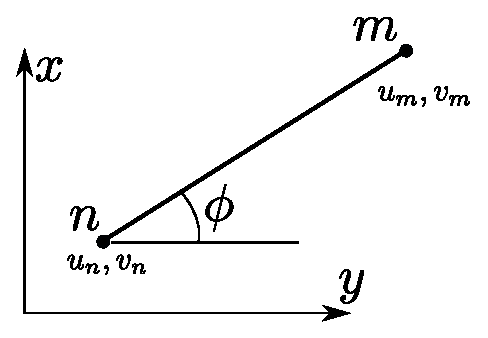
\includegraphics[width=7cm]{fig/rigidbarschematic.eps}
	\caption{Un rigid bar que une el nodo $n$ con el nodo $m$.}
	\label{fig:rigidbarschematic}
\end{figure}

El motivo del rigid bar es un elemento que \textit{no se acorta ni se alarga} con las fuerzas que transmite. Un usuario del método de elementos finitos podría pensar que alcanza con plantear dos ecuaciones $u_n=u_m$;$v_n=v_m$ sin embargo esto lograría que los nodos $n$ y $m$ se trasladen como un cuerpo rígido sin permitir rotaciones, efectivamente logrando una rigidez más alta que la propuesta en el motivo del rigid bar.

Si el rigid bar de la figura \ref{fig:rigidbarschematic} permite rotaciones sin acortarse, entonces la distancia que se mueve el nodo $m$ sobre el eje local $x'$ del rigid bar debe ser igual al del nodo $n$, dando una única ecuación
\[
u_n\cos\phi + v_n \sin\phi = u_m\cos\phi +v_m\sin\phi  
\]
esta restricción se puede agregar al sistema usando los multiplicadores de Lagrange o con el método del penal.


\subsection*{Rigid beam en el plano}
En el análisis ingenieril por FEA es común el uso de restricciones para modelar roscas, unir elementos con dof disimiles, etcætera. Para el segundo caso se puede usar un \textit{rigid link} (rigid beam) para transmitir rotaciones de un elemento/nodo con giro a un elemento sin giros en sus nodos, como podría ser el caso de unión viga-elemento 3D.

La formulación de un rigid link consiste en plantear ecuaciones de cinemática para una viga rígida (considerando desplazamientos pequeños). Los desplazamientos cartesianos del nodo slave serán condicionados por los giros del nodo master

\begin{align*}
	u_s &= u_m  + L_e \versor{v}_y\theta_m \\
	v_s &= v_m  - L_e \versor{v}_x \theta_m \\
	\theta_s &= \theta_m
\end{align*}
donde $L_e$ es la distancia entre nodo slave y master.

La formulación para un rigid link en el espacio puede ser deducida de la formulación RBE2 en el anexo de este documento planteando desplazamientos pequeños.

\section{Error}

Para calcular error ZZ primero se obtiene un campo de tensiones que ``mejor aproxima la solucion''{} llamado el \textbf{smoothed field} o campo suavizado ($\sigma^*$). Hay varios metodos para obtener $\sigma^*$, en este documento se va tratar el método de suavizado por elemento.

\subsection*{Element smoothing}
Se obtienen las tensiones sobre los puntos gauss superconvergentes mediante la ecuacion
\[
 \Cme{\sigmab^*}_i = \Mme{E} \Mme{B^*} \Cme{d}
\]
donde $\Mme{B^*}$ es evaluada sobre dichos puntos de gauss. Esto nos da el campo suavizado $\sigma^*$ del elemento. 

\subsection*{Error ZZ}
Para poder integrar las siguientes expresiones se tendrá que obtener $\Cme{\sigmab}_i$ sobre los puntos de cuadratura, es decir, habrá que interpolar el campo no-suavizado sobre los puntos gauss. En general no son idénticas las dos tensiones. Recordar que no tiene sentido obtener $\eta$ sobre un dominio que presenta discontinuidades de tensiones inherentes, como cambios abruptos de sección y cambio de material.
\[
\vvert{U}^2 = \sum^m_{i=1}\int_{v_e} \Cme{\varepsilonb}_i^T \ME \Cme{\varepsilonb}_i \di V
\]
donde $m$ es el numero de elementos del dominio donde se quiere calcular $\eta$.
\[
\vvert{e}^2=\sum_{i=1}^m \int_{v_e} \left( \Cme{\varepsilonb^*}_i - \Cme{\varepsilonb}_i\right)^T \ME \left( \Cme{\varepsilonb^*}_i - \Cme{\varepsilonb}_i\right) \di V
\]

\[
\vvert{e}^2=\sum_{i=1}^m \int_{v_e} \left( \Cme{\sigmab^*}_i - \Cme{\sigmab}_i\right)^T \ME ^{-1} \left( \Cme{\sigmab^*}_i - \Cme{\sigmab}_i\right) \di V
\]

El error relativo ($\eta$) esta comprendido entre 1 y 0. Un valor aceptable de $\eta$ suele ser tomado como $\eta\leq 0,05$ \citep{cook2007concepts}.
\[
\eta = \sqrt{\frac{\vvert{e}^2}{\vvert{e}^2+\vvert{U}^2}}
\]


\section{Transferencia de Calor}

Tenemos el flujo de calor que es $\underline{K} \nabla T$, la divergencia de esto es el flujo neto que pasa por un punto.
\[
\nabla(\underline{K} \nabla T)+Q=\rho c \frac{\partial T}{\partial \tau}
\] 

Ley de Newton: 
\[
q_{c}=h_{c}(s, T)\left(T-T_{\infty}\right)
\]

Ley de Stefan Boltzmann
\[
q_{r}=\varepsilon_{r} \sigma\left(T^{4}-T_{\infty}^{4}\right)
\]

Es mas complicado el tema de modelar temperaturas fijas e imponer calor transferido, pues son aseveraciones no tan reales como imponer desplazamiento cero sobre un apoyo y  fuerzas sobre vigas.

Para aplicar convección 

Hay una parte que depende de la temperatura interna, la parte que no depende la dejo como vector de cargas. La parte que depende la tengo que sumar a mi matriz de conductividades
\[
R_{C_{i}}=\oint_{\Gamma_{c o m v}} N_{i} h\left(T(x)-T_{f l}\right) d \gamma
\]

Lo escribe sebas: $kT=q_c = HT-RT_{fl} \longrightarrow (K-H)T = -R T_{fl}$

\[
\mathrm{Cargas:} R_{H} : \oint_{\Gamma_{c o n v}} N_{i} h T_{f l} d \gamma \qquad \qquad \mathrm{Conductividad:}  K : \oint_{\Gamma_{c m}} N_{i} h N_{j} d \gamma
\]


\subsection*{Resolución de problemas típico}

Condiciones de borde de temperatura. Idéntico a lo visto en la sección \ref{sec:desplzImpuestos}.

\[
\Cme{T_{\mathrm{x}}} = \Mme{K_{\mathrm{xx}}}^{-1} \left( \Cme{Q_\mathrm{x}}- \Mme{K_{\mathrm{xc}}}  \Cme{T_\mathrm{c}} \right)
\]
luego de obtener las temperaturas desconocidas se puede obtener el flujo desconocido (sobre los nodos conocidos):
\[
\Cme{Q_{\mathrm{c}}} = \Mme{K_{\mathrm{cx}}} \Cme{T_\mathrm{x}} + \Mme{K_{\mathrm{cc}}} \Cme{T_\mathrm{c}}  
\]
